\documentclass[letterpaper,11pt]{article}
%\documentclass[nojss]{jss}

\oddsidemargin 0.0in
\evensidemargin 0.0in
\textwidth 6.5in
%\headheight 0.0in

\usepackage{graphics}
\usepackage{amsmath}
\usepackage{indentfirst}
\usepackage{tabularx}
\usepackage{graphicx}
\usepackage{url}
\usepackage{appendix}
\usepackage{verbatim}
\usepackage{lscape}
\usepackage{rotating}
\usepackage{longtable}
\usepackage{apacite}


\DeclareMathOperator{\var}{var}
\DeclareMathOperator{\cov}{cov}

%\usepackage{Sweave}
\begin{document}

\title{An International Comparison of Private and Public Schools using Multilevel Propensity Score Methods and Graphics}
\author{Jason M. Bryer\\
\small{}jbryer@bryer.org\\
\small{}jbryer.github.com/multilevelPSA}
\date{\today}

\maketitle

\abstract{As can be seen from the recent Special Issue of \textit{Multivariate Behavioral Research} on propensity score methods the use of propensity score analysis (PSA) has gained increasing popularity for estimating causal effects in observational studies. However, PSA use with multilevel or clustered data has been limited, and to date there seems to have been no development of specialized graphics for such data. This paper will introduce the \texttt{multilevelPSA} package for R that provides cluster-based functions for estimating propensity scores (potentially for large datasets) as well as graphics to exhibit results for multilevel data. This work extends to the multilevel case the framework for visualizing propensity score analysis introduced by \citeA{PSAgraphics}. International data from the Programme for International Student Assessment, PISA, \cite{pisa} are comprehensively examined to compare private with public schools on reading, mathematics, and science outcomes after adjusting for covariate differences in the multilevel context.
\ \\ \ \\
\noindent Keywords: \textit{PSA, propensity score analysis, multilevel, graphics}}



\section{Introduction}

\section{Programme for International Student Assessment}


\section{Visualizing Multilevel Propensity Score Analysis}
The focus is on use of graphics for interpreting results of propensity score analyses where data are clustered. The goal is to use propensity score methods based on available covariates (all measures at the level of individuals) to adjust for differences between students in the two kinds of schools. Modern graphics permit learning how large extant differences are, and how results vary by countries, i.e. clusters.

\begin{figure}[ht]
\begin{center}
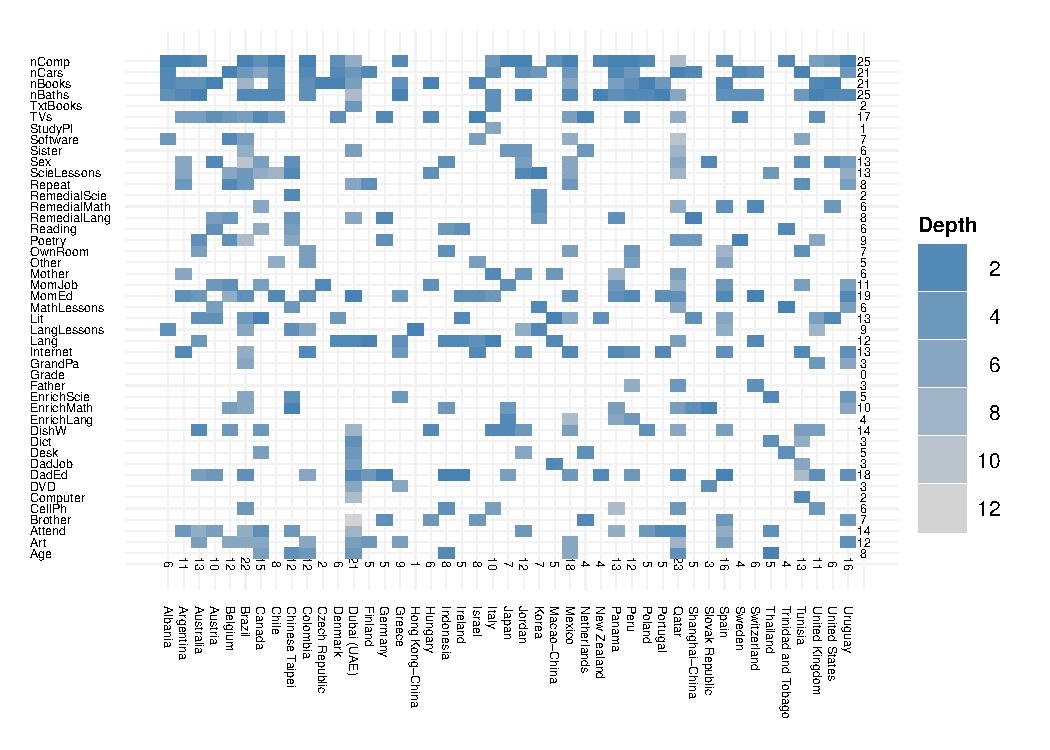
\includegraphics[width=6.5in]{figures/pisaTreeHeat}
\caption{Tree Heat of Multilevel Conditional Inference Trees}
\label{fig:math}
\end{center}
\end{figure}


\begin{figure}[ht]
\begin{center}
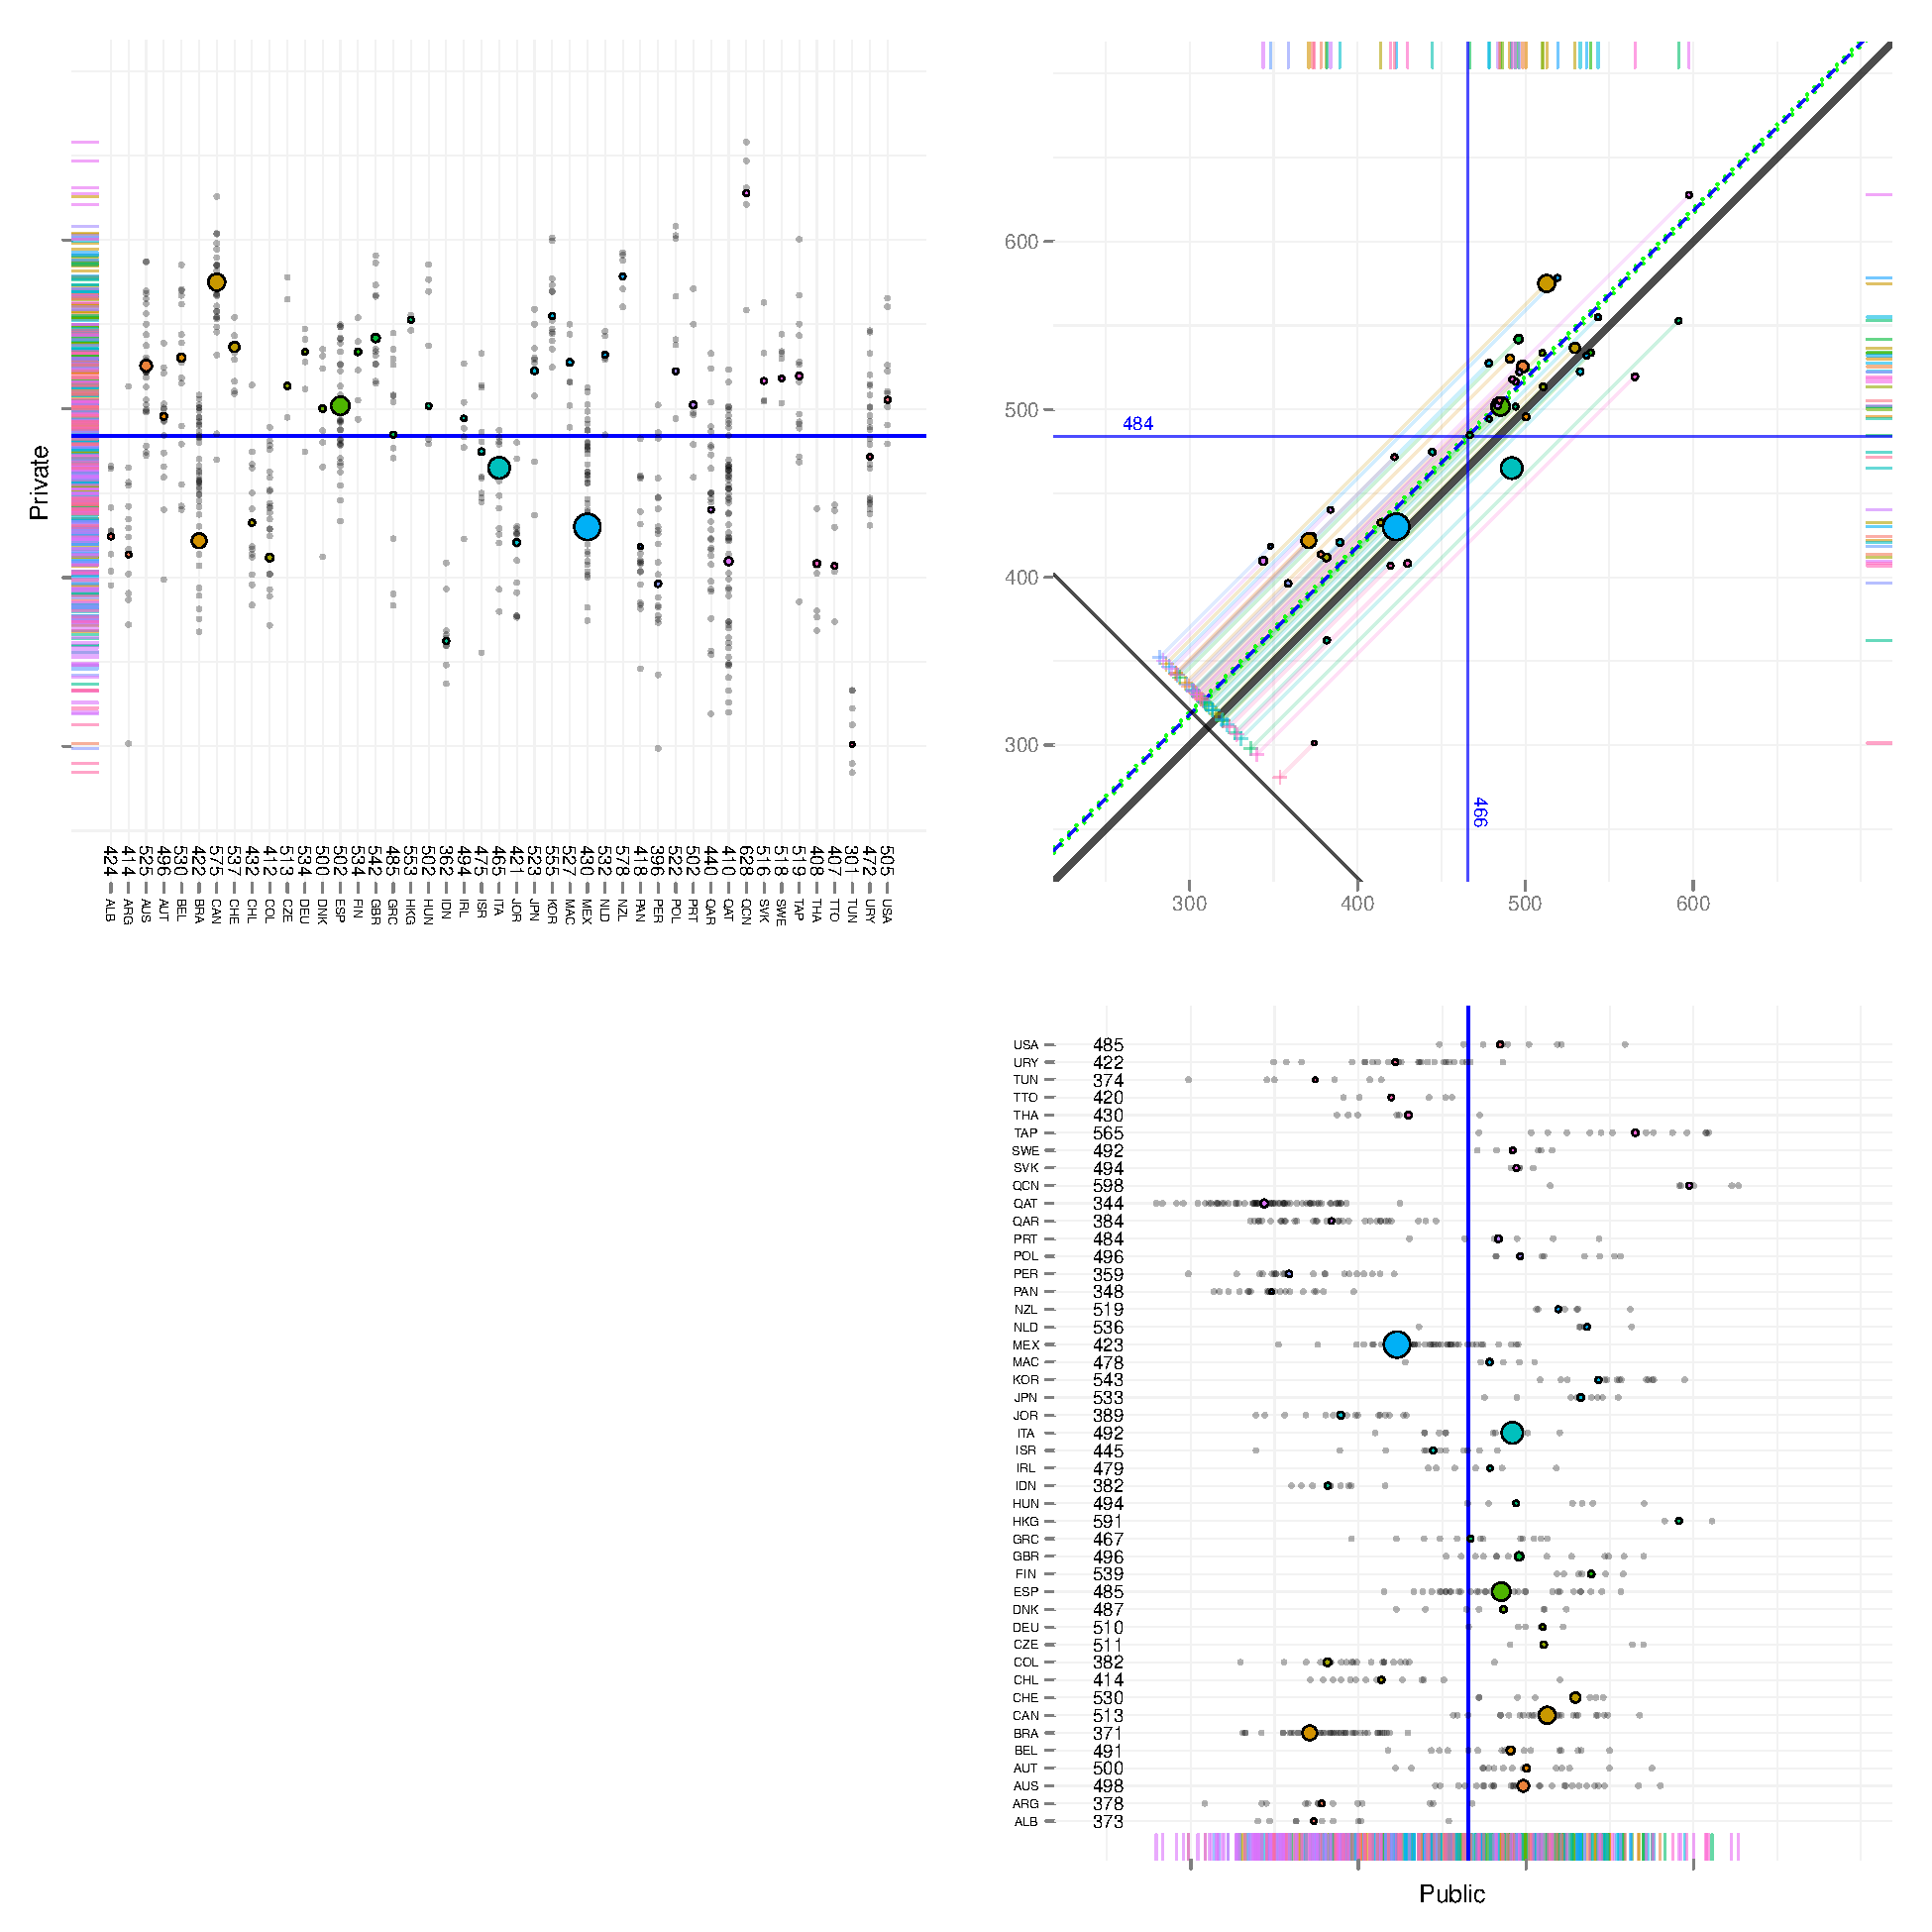
\includegraphics[width=6.5in]{figures/pisaMath.pdf}
\caption{Multilevel PSA Assessment Plot: Mathematics}
\label{fig:math}
\end{center}
\end{figure}

Figure 1 represents a multilevel assessment plot for the math assessment given at the end of secondary school. Coordinates for each point, one for each country, are overall adjusted means for stratifications based upon conditional inference trees of public and private schools on x- and y-axes. The size of each point (bubble) corresponds to the number of students sampled or tested within each country. Each point is projected, parallel to the identity line, to a �cross� on the line with slope -1 in the bottom left of the figure, to show the distribution of differences between public and private school scores across countries. The average difference and a confidence interval are also shown.

Figure 2 provides a more detailed representation of the distribution of differences. The x-axis corresponds to the difference scores and the y-axis to each country, for which differences are used to order results for countries. Blue dots correspond to the overall adjusted mean difference for each country along with the confidence intervals in green. The light grey dots correspond to differences for strata within each country. Similar to Figure 1, the vertical blue and green lines correspond to the overall adjusted mean difference and confidence interval, respectively.

\section{Results and Discussion}
Particularly for analyses of large data sets, focusing on statistical significance is limiting. As can readily be seen, overall results favor �private� over �public� schools, at least for end of secondary school math achievement. But the graphics, especially Figure 2, provide a more nuanced understanding of the nature and magnitude of adjusted differences for countries. Furthermore, the graphics are readily interpreted by a non-??technical audience. Broadly speaking, it is seen that modern graphics can enhance and extend conventional numerical summaries by focusing on details of what data have to say for multilevel comparisons of many countries based on PS methods.

\begin{figure}[ht]
\begin{center}
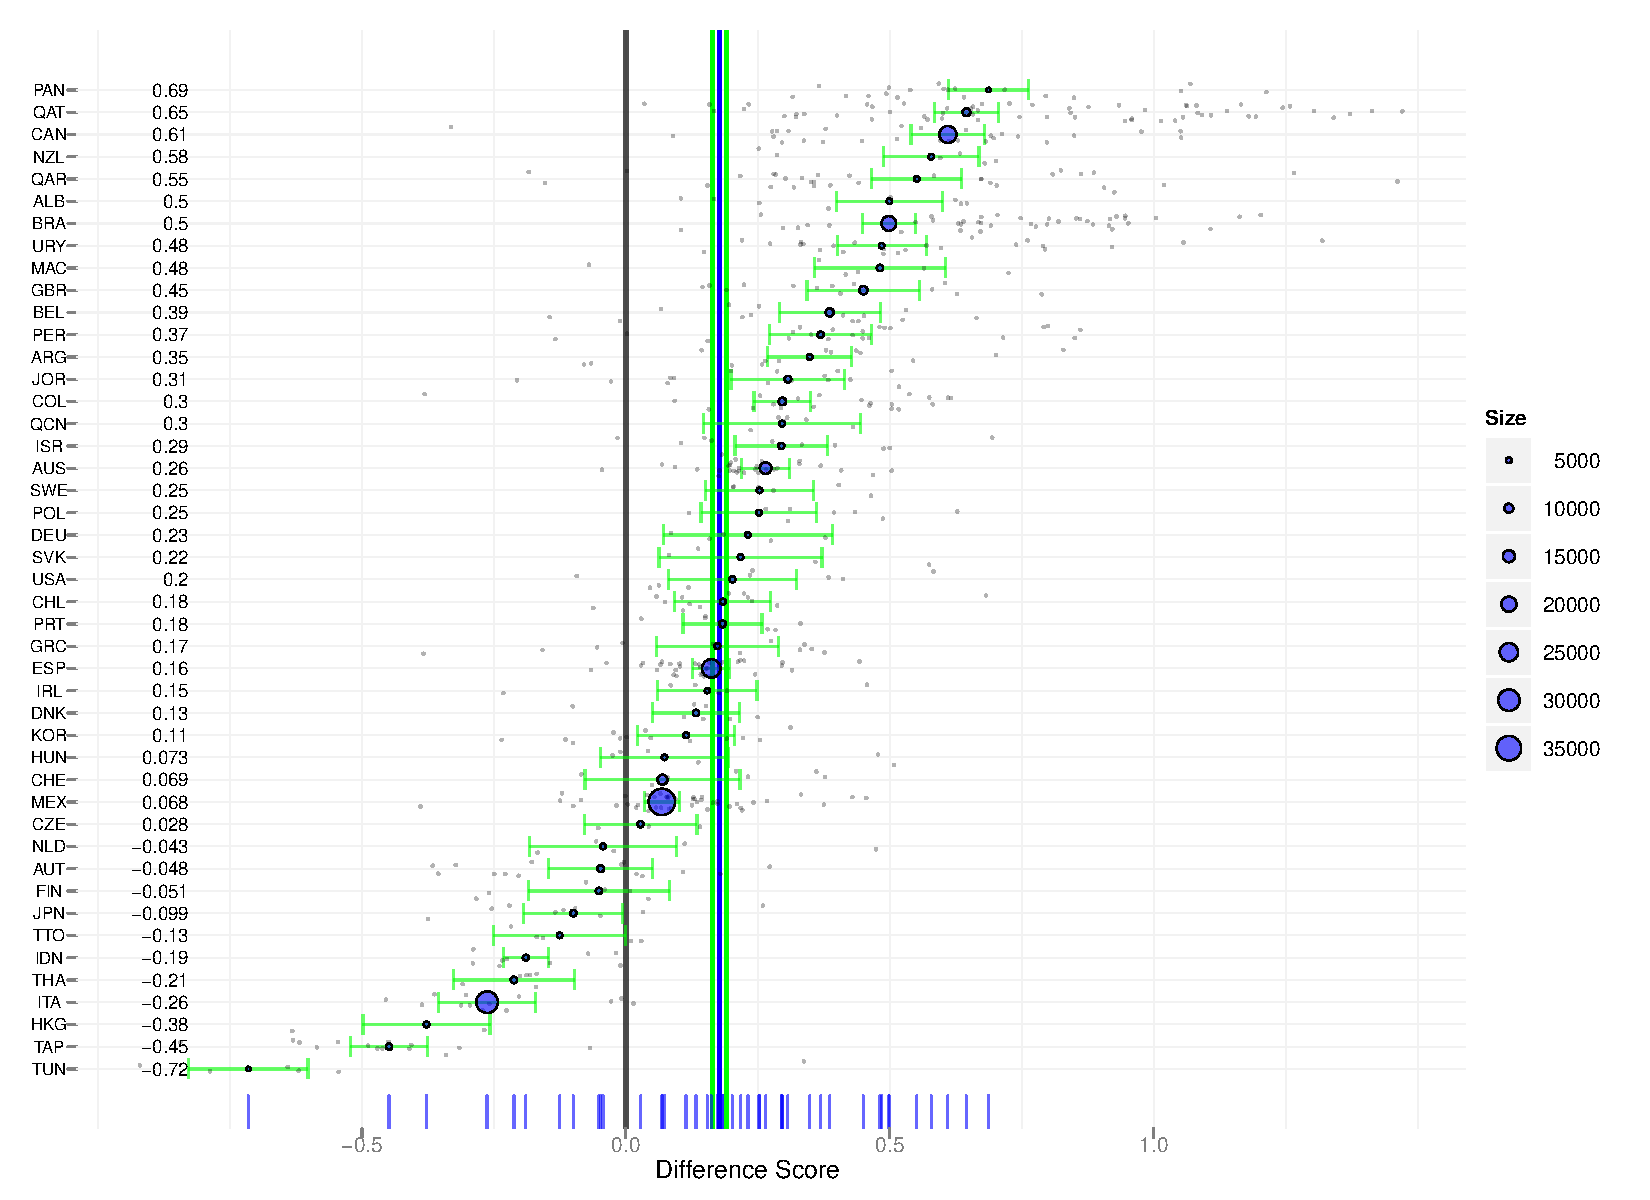
\includegraphics[width=6.5in]{figures/pisaMathDiff.pdf}
\caption{Multilevel PSA Difference Plot: Mathematics}
\label{fig:mathdiff}
\end{center}
\end{figure}


\section{Package Development}
The \texttt{multilevelPSA} package is hosted on github. The latest developmental version can be installed using the \texttt{devtools} package.


\bibliographystyle{apacite}
\bibliography{References}



\end{document}
